%!TEX root = ../../root.tex

We need to solve the general minimization problem:
\begin{equation}
	\epsilon = \min_\Theta \ell(\Theta)
\end{equation}
In particular, we are interested in the minimizer $\Theta$.
Finding minimizers for a general loss function is an open problem of the research area called \emph{optimization}. The optimization method depends on the specific property of the loss function, and, as we will see, there might sometimes be constraints on the parameters; nevertheless, we will mostly deal with unconstrained problems.

There are some classes of functions that are easier to minimize (or maximize) and the easiest set of functions is the set of convex functions, defined by \emph{Jensen's inequality}:
\begin{equation}\label{eq:convexity}
	f(\alpha x + (1 - \alpha)y) \leq \alpha f(x) + (1 - \alpha) f(y), \ \forall x,y \text{ and } \alpha \in [0,1]
\end{equation}
The inequality states that the convex transformation of a mean is less than or equal to the mean applied after convex transformation; for two points, it says that the secant line of a convex function lies above the graph of the function.
\begin{figure}[H]
	\centering
	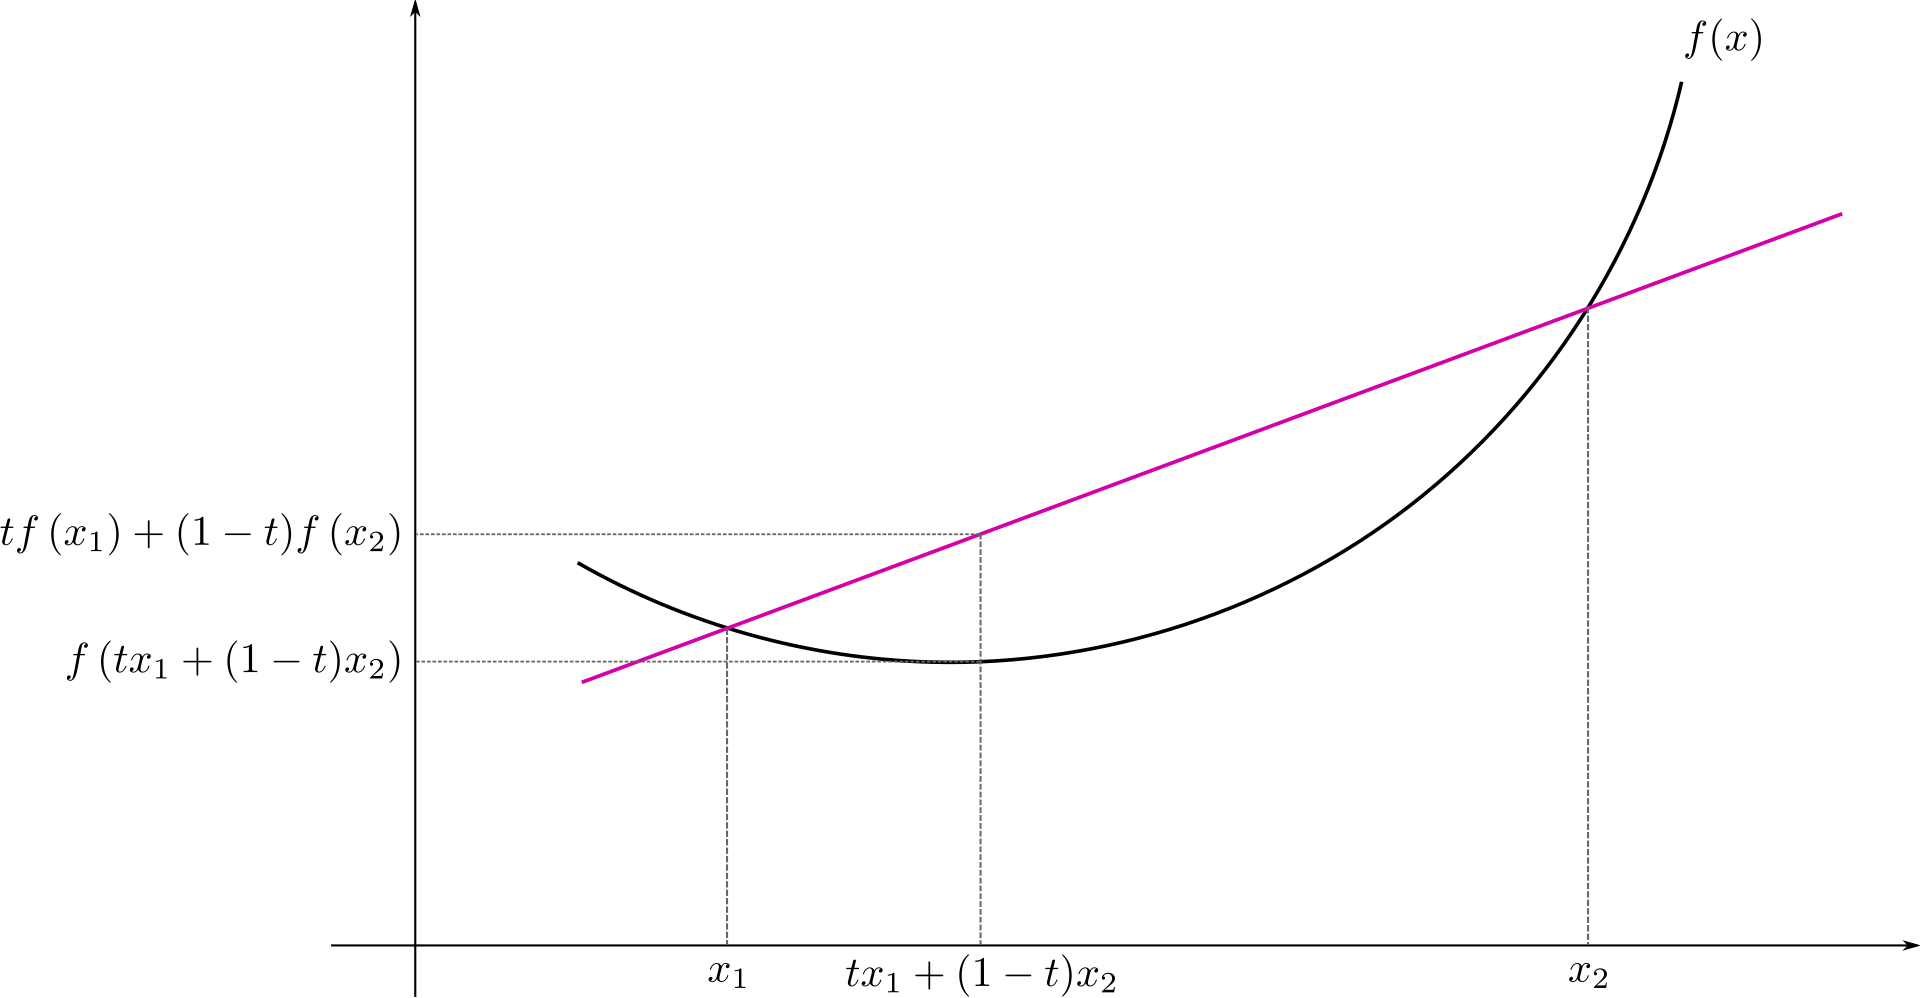
\includegraphics[width=.5\textwidth]{03/jensen}
	\caption{Jensen's inequality generalizes the statement that a secant line of a convex function lies above the graph.}\label{fig:jensen}	
\end{figure}

Why are these type of functions the easiest to minimize? Looking at the graph above, we can intuitively appreciate how there always exists a \emph{unique} minimum. If you recall some high school calculus you also know that the point where such minimum is achieved is the (again, unique) point where the \emph{derivative} of the function is zero.

Therefore, an important assumption that we often make is for the loss function $\ell$ to be differentiable, so we can compute its derivative $\dv{\ell}{x}$ at all points $x$. 

To explain this formally, let us write a different form of \cref{eq:convexity}:
\begin{equation}
	f(x + \alpha(y - x)) \leq (1 - \alpha)f(x) + \alpha f(y), \qquad \forall x,y \text{ and } \alpha \in (0,1)
\end{equation}
doing some algebraic manipulation we have:
\begin{align}
	&\frac{f(x + \alpha(y - x))}{\alpha} \leq \frac{(1 - \alpha)f(x) + \alpha f(y)}{\alpha} \\
	&\frac{f(x + \alpha(y - x))}{\alpha} \leq \frac{f(x)}{\alpha} - f(x) + f(y) \tag{expanding the product $(1 - \alpha)f(x)$} \\
	&\frac{f(x + \alpha(y - x)) - f(x)}{\alpha} + f(x) \leq f(y).
\end{align}
Now, we take the limit
\begin{equation}
	\lim_{\alpha \to 0} \frac{f(x + \alpha(y - x)) - f(x)}{\alpha} + f(x) \leq f(y)
\end{equation}
and notice how it resembles the definition of the derivative of a function, i.e. the limit of the difference quotient:
\begin{equation}
    \dv{f}{x} = \lim_{h \to 0} \frac{f(x + h) - f(x)}{h}
\end{equation}
To complete the expression we need a factor $(y - x)$:
\begin{equation}
	\lim_{\alpha \to 0} \frac{f(x + \alpha(y - x)) - f(x)}{\alpha (y - x)}(y - x) + f(x) \leq f(y) \qquad \forall x,y.
\end{equation}
Since $(y - x)$ is just a scalar we can move it out from the limit, so the entire limit represents the derivative of $f$:
\begin{equation}
	{\dv{f(x)}{x}} (y - x) + f(x) \leq f(y) \qquad \forall x,y.
\end{equation}
Notice that the left hand side of the inequality is just the $1$-st order Taylor approximation of $f$ at point $x$, \textit{i.e.} the best possible approximation of $f$ as a linear function at a given point $x$ and this would be the line that is tangent to the curve at that point.

\begin{figure}[H]
	\begin{center}
		\begin{overpic}
		[trim=0cm 0cm 0cm 0cm,clip,width=0.60\linewidth]{04/taylor}
			\put(1,30){\footnotesize $f(y)$}
			\put(70,15){\footnotesize $(x,f(x))$}
   			\put(90,29){\footnotesize $f(x) + \frac{df(x)}{dx}(y-x)$}
		\end{overpic}
	\end{center}
	\caption{Taylor approximation.}\label{fig:taylor}	
\end{figure}

Notice also that the slope of the line is given by the derivative, and that a flat line happens when the slope (the derivative) of the line is zero. Setting $\dv{f}{x} = 0$ we have that:
\begin{equation}\label{eq:minimizer}
	f(x) \leq f(y) \qquad \forall y
\end{equation}
and therefore $x$ is a global minimizer of $f$, as mentioned previously.

In general, if we want to find a minimizer for a convex function $f$ we just need to compute its derivative $\dv{f}{x}$, set it to zero and solve for $x$;  then as we have shown the point $x$ will satisfy \cref{eq:minimizer} and hence will be the global minimizer of the function.
